%% 
%% Copyright 2019-2024 Elsevier Ltd
%% 
%% This file is part of the 'CAS Bundle'.
%% --------------------------------------
%% 
%% It may be distributed under the conditions of the LaTeX Project Public
%% License, either version 1.3c of this license or (at your option) any
%% later version.  The latest version of this license is in
%%    http://www.latex-project.org/lppl.txt
%% and version 1.3c or later is part of all distributions of LaTeX
%% version 1999/12/01 or later.
%% 
%% The list of all files belonging to the 'CAS Bundle' is
%% given in the file `manifest.txt'.
%% 
%% Template article for cas-sc documentclass for 
%% double column output.

\documentclass[a4paper,fleqn]{cas-dc}


% If the frontmatter runs over more than one page
% use the longmktitle option.

%\documentclass[a4paper,fleqn,longmktitle]{cas-sc}

%\usepackage[numbers]{natbib}
%\usepackage[authoryear]{natbib}
%\usepackage[authoryear,longnamesfirst]{natbib}
\usepackage[numbers]{natbib}
\usepackage{xcolor}
\usepackage{booktabs} % Required for professional table lines
\usepackage{siunitx}  % Optional but highly recommended for numeric alignment
\usepackage{amsmath}
\usepackage{graphicx}
\usepackage{array}

%%%Author macros
\def\tsc#1{\csdef{#1}{\textsc{\lowercase{#1}}\xspace}}
\tsc{WGM}
\tsc{QE}
%%%

% Uncomment and use as if needed
%\newtheorem{theorem}{Theorem}
%\newtheorem{lemma}[theorem]{Lemma}
%\newdefinition{rmk}{Remark}
%\newproof{pf}{Proof}
%\newproof{pot}{Proof of Theorem \ref{thm}}

\begin{document}
	\let\WriteBookmarks\relax
	\def\floatpagepagefraction{1}
	\def\textpagefraction{.001}
	
	% Short title
	\shorttitle{TI and RI for CNN Reliability Evaluation}    
	
	% Short author
	\shortauthors{Mehedi et al}  
	
	% Main title of the paper
	\title [mode = title]{Beyond Accuracy: Explainable Trustworthy Index and Explainable Robustness Index for Evaluating CNN}  
	
	% Title footnote mark
	% eg: \tnotemark[1]
	%\tnotemark[1] 
	
	% Title footnote 1.
	% eg: \tnotetext[1]{Title footnote text}
	%\tnotetext[1]{} 
	
	% First author
	%
	% Options: Use if required
	% eg: \author[1,3]{Author Name}[type=editor,
	%       style=chinese,
	%       auid=000,
	%       bioid=1,
	%       prefix=Sir,
	%       orcid=0000-0000-0000-0000,
	%       facebook=<facebook id>,
	%       twitter=<twitter id>,
	%       linkedin=<linkedin id>,
	%       gplus=<gplus id>]
	
	\author[1]{Ragib Mehedi}[orcid=0009-0003-1555-7338]
	\ead{ragib6627@gmail.com}
	\cormark[1]
	\credit{Conceptualization, Methodology, Software, Investigation, Formal analysis, Writing – Original Draft, Writing – Review \& Editing}
	
	\author[1]{Azmain Inquaid Haque}
	\ead{azmaininquaidhaque@gmail.com}
	\credit{Investigation, Data Curation, Software, Validation}
	
	\author[2]{Md. Nazmul Abdal}
	\ead{nazmul.abdal@ulab.edu.bd}
    \ead[url]{https://ulab.edu.bd/faculty/md-nazmul-abdal}
	\credit{Data Curation}
	
	
	\author[1]{Abdullah Al Noman}
	\ead{noman@cse.ku.ac.bd}
    \ead[url]{https://ku.ac.bd/discipline/cse/faculty/noman}
	\cormark[1]
	\credit{Supervision, Writing – Review \& Editing}
	% Corresponding author indication
	
	
	\author[1]{Md. Zahidul Islam}
	\ead{zahid@cse.ku.ac.bd}
    \ead[url]{https://ku.ac.bd/discipline/cse/faculty/zahid}
	\credit{Supervision, Writing – Review \& Editing }
	
	\affiliation[1]{ organization={Computer Science and Engineering Discipline, Khulna University}, city={Khulna}, postcode={9208}, country={Bangladesh} } 
	\affiliation[2]{ organization={Department of Computer Science and Engineering, University of Liberal Arts Bangladesh}, city={Dhaka}, postcode={1207}, country={Bangladesh} }
	
	\cortext[1]{Corresponding author}
	
	% For a title note without a number/mark
	%\nonumnote{}
	
	% Here goes the abstract
	
	% Define the command \mycom that takes 1 argument (#1) and makes it green
	\newcommand{\zahid}[1]{{\color{green}#1}}
	
	\begin{abstract}
	Deep neural networks often achieve high classification accuracy. Despite high accuracy, the reliability of CNN models remains a concern. Sometimes CNN models may rely on background or irrelevant features, undermining trustworthiness. Besides, with the use of perturbations, models' accuracy and object reliance may decline. Such degradation raises questions about their robustness. In this research, we have proposed two novel evaluation metrics: the \textbf{Explainable Trustworthy Index (ETI)} and the \textbf{Explainable Robustness Index (ERI)}. ETI combines accuracy with the \textbf{Localization Mask Overlap Score (LMOS)}, which measures the proportion of Grad-CAM salient pixels that fall within the ground-truth object regions. A model with high ETI clearly indicates that both its accuracy and object reliance are high and satisfactory. ERI extends this to perturbed inputs by jointly evaluating accuracy stability and LMOS stability.  Like ETI, a model with high ERI indicates that both its accuracy and object focus remain stable under the use of perturbations. We have used eight CNN architectures on four datasets and nine perturbations (e.g., noise, blur, motion blur, occlusion) to calculate ETI and ERI. We have demonstrated that high accuracy sometimes does not guarantee high ETI or ERI. For instance, on the EPLI dataset, Custom CNN has achieved 99.45\% accuracy but the lowest ETI (0.5922) due to poor object localization. It has also provided the lowest ERI. ETI and ERI provide a more holistic assessment of model reliability for safety-critical applications.
	\end{abstract}
	
	% Use if graphical abstract is present
	%\begin{graphicalabstract}
	%\includegraphics{}
	%\end{graphicalabstract}
	
	% Research highlights
	%\begin{highlights}
	%	TBD
	%\end{highlights}
	
	
	% Keywords
	% Each keyword is seperated by \sep
	\begin{keywords}
		Explainable AI (XAI), Trustworthiness, Robustness, CNN, Grad-CAM, Perturbation Analysis, Plant Leaf Classification
	\end{keywords}
	
	\maketitle
	
	
	\section{Introduction}
	\label{sec:introduction}
	%\zahid{\textbf{We need to explain CNN reliability and XAI from title. }}
	Convolutional Neural Networks (CNNs) have achieved remarkable performance in a wide range of domains such 
    as medical imaging, agriculture, and astronomy, where predictions support important decision-making processes
	\cite{r1}\cite{r2}\cite{r3}\cite{r4}. In such applications, classification accuracy is an essential performance
	measure, but accuracy alone does not necessarily indicate whether a model is reliable. A CNN model is considered more
	reliable when its predictions are grounded in task-relevant visual features rather than spurious 
	correlations\cite{r5}.
	\zahid{Wu, J., Kang, W., Tang, H., Hong, Y., \& Yan, Y. (2024). On the faithfulness of vision transformer explanations. 2024 IEEE/CVF Conference on Computer Vision and Pattern Recognition (CVPR), 10936–10945. https://doi.org/10.1109/cvpr52733.2024.01040

	Zafar, A. (2026). Evaluating visual grounding in multimodal medical reasoning. International Conference on Learning Representations (ICLR) Workshop} already added 
	\\

	 \zahid{provide one or model example images from your dataset with sample images and explain it.} \\

	Therefore, beyond predictive accuracy, models must be quantitatively evaluated to determine whether 
	their predictions depend on task-relevant regions rather than irrelevant background cues. % continuing introducing the problem 
	Despite excellent accuracy, a model may not provide reliable predictions. Explainability methods, such as 
	Grad-CAM \cite{r6}, show that a model may rely mainly on  background and irrelevant regions instead of 
	focused objects \cite{ r7, r8}. This raises questions about reliability and trustworthiness. 
	%\zahid{we are not working to imrpove relaiability??}
	
	%\zahid{Traditional CNN model evaluation meausres fail to indicate the reliability of the correspoinding model.}
	
	% problem of domain-shift 
	% Model behavior can also change due to perturbations commonly occur in real-world such as during image aquisition. 
	%Model behavior can shift due to real-world perturbations. 
	%, such as those occurring during image acquisition. 
	%Common distortions (e.g., noise, blur, brightness/contrast adjustments, hue shifts, compression, and occlusion) can alter both CNN accuracy and the specific visual regions driving model predictions.
	%Common changes such as noise, blur, brightness variation, hue shift, contrast modification, compression, and occlusion can alter both classification performance and the visual regions emphasized by a CNN \cite{r4,r5,r9}.  
	%That is, a model maintaining relatively high accuracy under perturbations may become visually inconsistent  \cite{r4,r5,r9}. 
	Model behavior can shift due to real-world perturbations e.g., noise, blur, lighting shifts, compression, 
	and occlusion. These distortions can alter both CNN accuracy and the visual regions driving predictions. 
	Consequently, even when a model maintains relatively high accuracy under perturbations, 
	its underlying visual explanations may still become inconsistent \cite{r5,r9}. Conventional robustness 
	evaluation methods are primarily based on accuracy change under perturbation. They do not capture whether the model
	maintains consistent reliance on task-relevant regions under perturbed conditions. These observations motivate an evaluation 
	ramework that considers both predictive behavior and explanation behavior.
	% above paragraph is good to go
	
	% moving towards the generic solution
	Explainable Artificial Intelligence (XAI) provides a framework for examining visual evidences used by CNNs for their predictions. 
	In particular, Grad-CAM generates class-discriminative heatmaps that highlight image regions contributing to a model's prediction
	 \cite{r6}. The faithfulness of such explanations is an important consideration, since explanation scores should meaningfully 
	reflect the influence of the corresponding image regions on the model’s prediction \cite{r10}. Such explanations can reveal whether a 
	model achieves high classification accuracy by focusing substantially on 
	background or other irrelevant regions rather than target objects. Previous studies have shown that background information and 
	spurious correlations can influence deep neural network decisions and may lead to shortcut learning \cite{r11, r12, r13} %\zahid{add more relevent refs}. 
	Consequently, a highly accurate model does not confirm that the predictions are made on appropriate object-level information. 
	This creates an important distinction between predictive performance and explainable reliability. %Now it is necessary to evaluate whether a model's accuracy is based on task-relevant regions. 
	This is the motivation for evaluating a framework that combines accuracy and object focus.
	% above paragraph sounds okay
		
	% proposed solution
	%To address this limitation (\zahid{we did not say the limitation yet}), 
	We have proposed two novel evaluation metrics: Explainable Trustworthy Index (ETI) and Explainable Robustness Index (ERI) using XAI methods. 
	Our objective is not to modify or improve CNN models, rather to provide quantitative measures for evaluating and comparing their
	reliability and robustness. 
	ETI measures baseline reliability on unperturbed images by jointly evaluating classification accuracy and object-focused explanation quality. 
	In contrast, ERI measures robustness to input perturbations by assessing whether accuracy and explanation quality remain consistent with clean-image behavior.
	%ETI evaluates model reliability on clean, unperturbed images by jointly considering classification accuracy and object-focused explanation quality. 
	%In contrast, ERI evaluates robustness under input perturbations
	%by measuring whether both classification performance and
	%object-focused explanations remain stable compared with
	%clean-image behavior. 
	In essence, ETI and ERI address two different questions: ETI asks ``Whether a model is accurate and appropriately focused on the target object 
	under normal conditions?'', whereas ERI asks ``Whether these properties remain stable when the input is perturbed?''
	
	%We highlight the importance of object reliability (\zahid{is this correct? or model reliability?}) as well as accuracy. 
	%TI integrates accuracy and object reliability (\zahid{??}) in clean images. 
	%RI measures the robustness under various perturbations. \zahid{need to define robustness with ref}
	%Robustness measures how close the model's accuracy and explanations (object reliance) under perturbation remain to the outputs on clean images (\zahid{good but not clear - remember if you have to think to understand a sentence - you should probably rewrite it!}). 
	
	%The proposed measures TI and RI rely on the fact that \textit{how much a model's predictions rely on real objects instead of the background}. 
	%We introduce a new score named LMOS (Localization Mask	Overlap Score) to indicate this fact. 
	
	We introduce the Localization Mask Overlap Score (LMOS) to quantify object-focused explanation quality. 
	For each test image, we create a ground-truth mask for the target object excluding the background. 
	We use Grad-CAM \cite{r6} to identify the image regions contributing to the model's prediction.
	LMOS quantifies the proportion of the model's decision-relevant activation that overlaps with the annotated target-object region. 
	%Grad-CAM highlights key predictive regions using a color heatmap, where red and yellow denote the highest activation and strongest influence on the decision.
	It is observed that in Grad-CAM visualizations, red and yellow regions in images are activated most i.e., red and yellow have 
	greater influence than other colors on models' predictions \cite{r14} \cite{r15}. So we consider them as decision-relevant regions. \zahid{any ref to this??}. 
   	We integrate this principle into LMOS; a higher LMOS value indicates that a larger proportion of the model's highlighted regions falls within the target object boundary rather than the background.
	%So we consider them as decision-relevant. Therefore, a higher LMOS indicates that a larger proportion of the model's highlighted regions is located within the target object rather than outside it. LMOS provides a quantitative measure that can be compared across CNN architectures and datasets.
	
	%As red and yellow regions of the Grad-CAM visualization have stronger influence than other regions for predictions, we consider them as decision-relevant. \zahid{why do we need this sentence?}
	
	%LMOS defines when the model relies on something to make decisions, what ratio of that reliance falls on focus objects. \zahid{not clear}
	
	%A model has high accuracy but low LMOS may be affected by shortcut learning, overfitting, bias, and reliance on background features. \zahid{can we show this - i.e., a model having high acc but low LMOS and has one or more of the mentioned problems?}
	% \textbf{A model is trustworthy if it has high accuracy and high LMOS. 
	% 	Similarly, a model is considered robust under perturbations if it maintains high accuracy stability, and high LMOS stability under perturbations. }
	
	%\zahid{need clear distinctions between EI and RI - what EI shows must be different than RI}
	
	%Models with high TI is considered reliable as both the model accuracy and object reliance are high. 
	%Models with moderate to low TI means its accuracy or object focus, or both, are low and limited. 
	
	To comprehensively evaluate the proposed metrics, we conduct experiments using four public real-world datasets comprising two leaf image datasets:  EPLI \cite{r16}, BDML\cite{r17} and two flower image datasets: FLRS \cite{r18}, FR \cite{r19}. 
	Eight CNN architectures are trained and evaluated on the datasets. %For the test images, target-object masks are manually annotated to provide the spatial reference required for LMOS calculation. 
	%Grad-CAM explanations are generated for both clean and perturbed test images. 
	We evaluate nine perturbations, including Gaussian noise, Gaussian blur, brightness adjustment, hue shift, contrast adjustment, gamma correction, motion blur, JPEG compression, and random occlusion \zahid{cite all the methods}. 
	For each CNN architecture, ETI is calculated on clean images, while ERI is calculated from accuracy stability and LMOS stability across the evaluated perturbations.
	
	We empirically demonstrate the importance of combining accuracy with LMOS in ETI. 
	For example, a custom CNN achieves 99.45\% classification accuracy on the EPLI dataset, yet its mean LMOS is only 0.1900, resulting in the lowest ETI score of 0.5922 among the evaluated models. Its LMOS is only 0.1900, indicating that only 19.00\% of its decision-relevant activation, on average, falls within the annotated target-object regions, while the remaining 81.00\% lies outside these regions. \zahid{what is the consequence??  e.g., XX\% of predictions are based on background??}
	In contrast, the MobileNetV2 also achieves 99.45\% accuracy but obtains a substantially higher mean LMOS of 0.7765, indicating that 77.65\% of its decision-relevant activation falls within the target-object regions, with only 22.35\% outside them and an ETI of 0.8855. \zahid{what is the consequence?? e.g., XX\% of predictions are based on background, must be less than custom CNN??}
	This demonstrates that models with similar high accuracy can exhibit substantially different levels of object-focused reliance and the model with higher LMOS should be selected for real-world deployment. 
	%A high accuracy score alone therefore cannot distinguish between a model that makes predictions while focusing on the target object and a model that achieves similar accuracy while emphasizing regions outside the target object. 
	%Importantly, low LMOS does not by itself indicate shortcut learning, bias, or overfitting; rather. It provides quantitative evidence that the model's decision-relevant activation is insufficiently aligned with the target object, which demands further investigation.
	Importantly, a low LMOS score does not inherently denote shortcut learning or overfitting, but rather quantifies the extent to which a model's salient activations diverge from the target object.
	
	ERI combines \emph{accuracy stability} and \emph{LMOS stability} to provide a joint measure of explainable robustness. 
	This distinction is important because predictive stability and explanation stability are not correlated. 
	For example, on the EPLI dataset, the Custom CNN under contrast perturbation maintains relatively high accuracy stability of 0.8494 but has substantially lower LMOS stability of 0.4545. This indicates that, although its predictive performance remains comparatively stable, its object-focused explanation changes substantially relative to the clean-image condition. 
	Conversely, ResNet50 under the same perturbation exhibits relatively low accuracy stability of 0.4599 but higher LMOS stability of 0.7830, indicating that its object-focused explanation remains comparatively more consistent despite a larger change in predictive performance. 
	\zahid{what is the consequence of this??}
	These demonstrate that accuracy stability alone cannot fully characterize robustness: a model may preserve its predictive performance while substantially changing its object-focused behavior, or it may preserve its visual focus while its predictive performance deteriorates. 
	%ERI therefore evaluates these two complementary dimensions jointly.
	
	
	%The significance of ETI and ERI lies in their ability to capture specific aspects of CNN reliability and robustness that conventional accuracy-based evaluation overlook. 
	%A higher ETI indicates stronger joint performance in classification accuracy and object-focused explanation alignment under clean inputs, whereas a lower ETI indicates weaker performance in one or both of these dimensions. 
	%ERI extends this evaluation to perturbed inputs by jointly considering the stability of predictive performance and object-focused explanations relative to clean-image behavior. 
	%We note that a higher ETI or ERI should not be interpreted as higher overall trustworthiness and robustness. 
	%Trustworthiness and robustness may involve many other factors beyond the properties evaluated in this work. 
	%Instead, we focus specifically on predictive accuracy, object-focused explanation quality, and their stability under perturbations. 
	%Together, ETI and ERI provide complementary measures for comparing CNN models beyond conventional accuracy-based evaluation methods.
	The significance of ETI and ERI lies in their ability to capture key dimensions of CNN reliability and robustness that standard accuracy metrics overlook. 
	However, a high ETI or ERI score should not be equated with overall model trustworthiness, which encompasses broader factors beyond the scope of this work. 
	Rather, these metrics focus specifically on predictive accuracy, object-focused explanation quality, and their stability under input perturbations - offering complementary criteria for evaluating CNN models beyond conventional accuracy benchmarks.
	
	%To evaluate the robustness of the models, we have applied nine perturbations (noise, blur, hue, occlusion, etc.) to the test images and then calculated accuracy and LMOS scores after each perturbation. 
	
	%The mean LMOS stability under a perturbation has been obtained by averaging the image-wise LMOS stability values across all test samples. 
	%Then, ERI under a perturbation has been calculated as the mean of both stabilities. 
	%Finally, the mean ERI across all perturbations has been calculated and a ranking has been made according to the mean ERI. 
	%Like ETI, a model with hight ERI indicates that both its accuracy and object focus remain stable under the use of perturbations. 
	%A moderate/low ERI reveals that its accuracy, or focus on object, or both change with the use of perturbations.





% EgyPLI idx = 11
% BDML idx = 10
\begin{table*}[htbp]
\centering
\renewcommand{\arraystretch}{1.5}
\caption{Grad-CAM visualization on EPLI}
\label{tab:model_robustness}

\resizebox{\textwidth}{!}{%
\begin{tabular}{C{3.5cm} C{2.2cm} C{2.2cm} C{2.2cm} C{2.2cm} C{2.2cm} C{2.2cm} C{2.2cm}}
\hline

\textbf{Model} &
\textbf{Original} &
\textbf{Segmented} &
\textbf{Clean} &
\textbf{Hue} &
\textbf{Blur} &
\textbf{Contrast} &
\textbf{Compression}
\\
\hline

\begin{tabular}[c]{l}
Model: Xception \\
Accuracy: 99.45\% \\
Mean LMOS: 0.7638\\
ETI: 0.8791 \\
ERI: 0.9346
\end{tabular}
&
\begin{tabular}[c]{c}
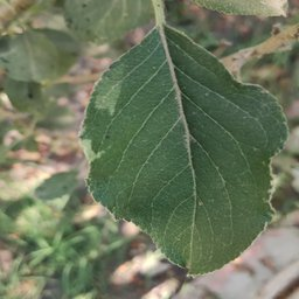
\includegraphics[width=2cm]{images/Introduction/EgyPLI/Xception/IMG_20240710_162039_original.png} \\[-1mm]
\scriptsize Apple (EPLI) % Original image
\end{tabular}
&
\begin{tabular}[c]{c}
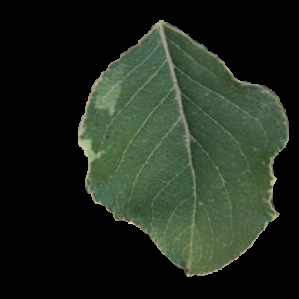
\includegraphics[width=2cm]{images/Introduction/EgyPLI/Xception/IMG_20240710_162039_segmented.png} \\[-1mm]
\scriptsize %Segmented image
\end{tabular}
&
\begin{tabular}[c]{c}
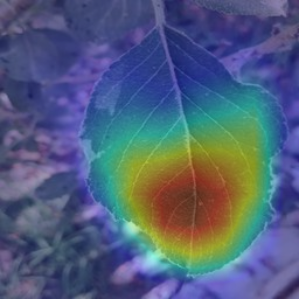
\includegraphics[width=2cm]{images/Introduction/EgyPLI/Xception/IMG_20240710_162039_clean.png} \\[-1mm]
\scriptsize LMOS: 1.00
\end{tabular}
&
\begin{tabular}[c]{c}
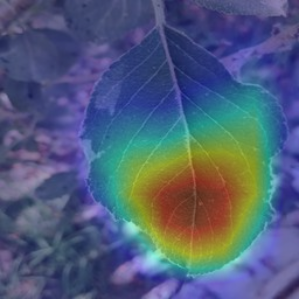
\includegraphics[width=2cm]{images/Introduction/EgyPLI/Xception/IMG_20240710_162039_hue.png} \\[-1mm]
\scriptsize LMOS: 1.00
\end{tabular}
&
\begin{tabular}[c]{c}
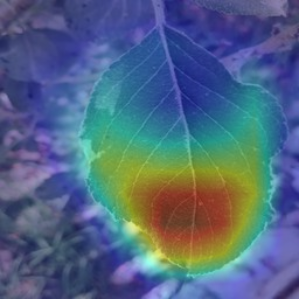
\includegraphics[width=2cm]{images/Introduction/EgyPLI/Xception/IMG_20240710_162039_blur.png} \\[-1mm]
\scriptsize LMOS: 1.00
\end{tabular}
&
\begin{tabular}[c]{c}
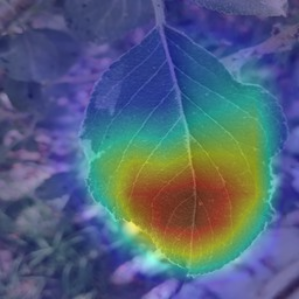
\includegraphics[width=2cm]{images/Introduction/EgyPLI/Xception/IMG_20240710_162039_contrast.png} \\[-1mm]
\scriptsize LMOS: 1.00
\end{tabular}
&
\begin{tabular}[c]{c}
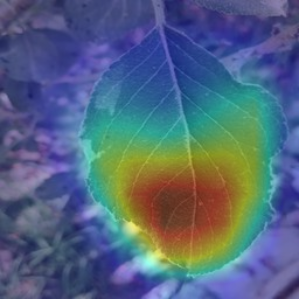
\includegraphics[width=2cm]{images/Introduction/EgyPLI/Xception/IMG_20240710_162039_compression.png} \\[-1mm]
\scriptsize LMOS: 1.00
\end{tabular}
\\
\hline

\begin{tabular}[c]{l}
Model: Custom CNN \\
Accuracy: 99.45\% \\
Mean LMOS: 0.1900\\
ETI: 0.5922 \\
ERI: 0.7944
\end{tabular}
&
\begin{tabular}[c]{c}
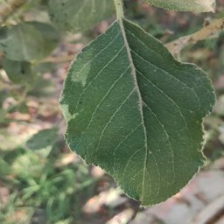
\includegraphics[width=2cm]{images/Introduction/EgyPLI/Custom_CNN/IMG_20240710_162039_original.png} \\[-1mm]
\scriptsize Apple (EPLI) % Original image
\end{tabular}
&
\begin{tabular}[c]{c}
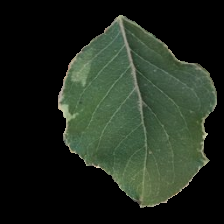
\includegraphics[width=2cm]{images/Introduction/EgyPLI/Custom_CNN/IMG_20240710_162039_segmented.png} \\[-1mm]
\scriptsize %Segmented image
\end{tabular}
&
\begin{tabular}[c]{c}
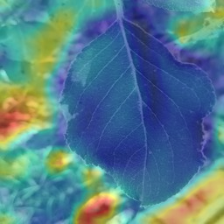
\includegraphics[width=2cm]{images/Introduction/EgyPLI/Custom_CNN/IMG_20240710_162039_clean.png} \\[-1mm]
\scriptsize LMOS: 0.00
\end{tabular}
&
\begin{tabular}[c]{c}
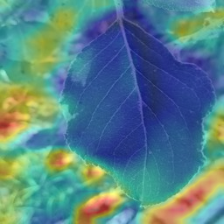
\includegraphics[width=2cm]{images/Introduction/EgyPLI/Custom_CNN/IMG_20240710_162039_hue.png} \\[-1mm]
\scriptsize LMOS: 0.00 
\end{tabular}
&
\begin{tabular}[c]{c}
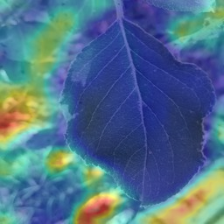
\includegraphics[width=2cm]{images/Introduction/EgyPLI/Custom_CNN/IMG_20240710_162039_blur.png} \\[-1mm]
\scriptsize LMOS: 0.00
\end{tabular}
&
\begin{tabular}[c]{c}
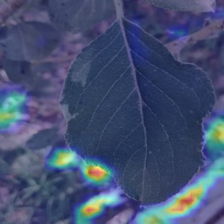
\includegraphics[width=2cm]{images/Introduction/EgyPLI/Custom_CNN/IMG_20240710_162039_contrast.png} \\[-1mm]
\scriptsize LMOS: 0.00
\end{tabular}
&
\begin{tabular}[c]{c}
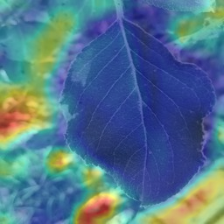
\includegraphics[width=2cm]{images/Introduction/EgyPLI/Custom_CNN/IMG_20240710_162039_compression.png} \\[-1mm]
\scriptsize LMOS: 0.00
\end{tabular}
\\
\hline


\begin{tabular}[c]{l}
Model: Xception \\
Accuracy: 95.05\% \\
Mean LMOS: 0.7800 \\
ETI: 0.8653 \\
ERI: 0.8982
\end{tabular}
&
\begin{tabular}[c]{c}
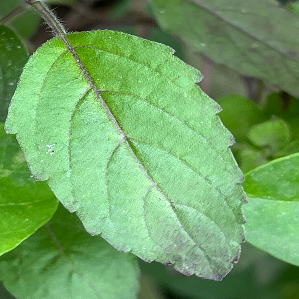
\includegraphics[width=2cm]{images/Introduction/BDML/Xception/IMG_9012_original.png} \\[-1mm]
\scriptsize Ocimum tenuiflorum (BDML) % Original image
\end{tabular}
&
\begin{tabular}[c]{c}
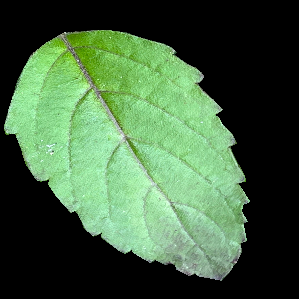
\includegraphics[width=2cm]{images/Introduction/BDML/Xception/IMG_9012_segmented.png} \\[-1mm]
\scriptsize %Segmented image
\end{tabular}
&
\begin{tabular}[c]{c}
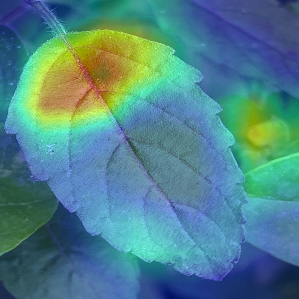
\includegraphics[width=2cm]{images/Introduction/BDML/Xception/IMG_9012_clean.png} \\[-1mm]
\scriptsize LMOS: 1.00
\end{tabular}
&
\begin{tabular}[c]{c}
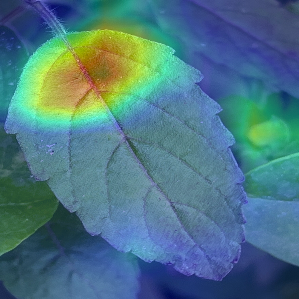
\includegraphics[width=2cm]{images/Introduction/BDML/Xception/IMG_9012_hue.png} \\[-1mm]
\scriptsize LMOS: 1.00
\end{tabular}
&
\begin{tabular}[c]{c}
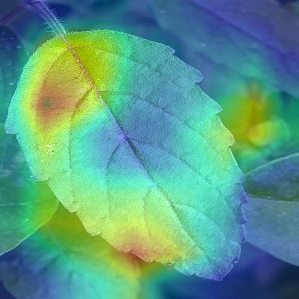
\includegraphics[width=2cm]{images/Introduction/BDML/Xception/IMG_9012_blur.png} \\[-1mm]
\scriptsize LMOS: 0.903
\end{tabular}
&
\begin{tabular}[c]{c}
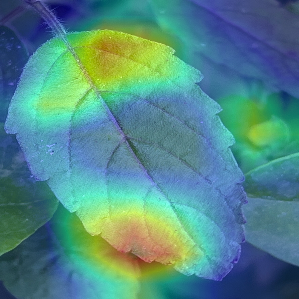
\includegraphics[width=2cm]{images/Introduction/BDML/Xception/IMG_9012_contrast.png} \\[-1mm]
\scriptsize LMOS: 0.812
\end{tabular}
&
\begin{tabular}[c]{c}
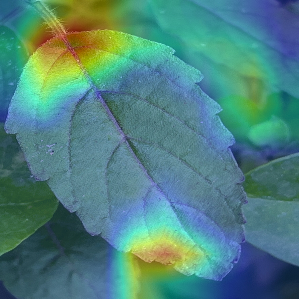
\includegraphics[width=2cm]{images/Introduction/BDML/Xception/IMG_9012_compression.png} \\[-1mm]
\scriptsize LMOS: 0.785
\end{tabular}
\\
\hline

\begin{tabular}[c]{l}
Model: Inception V3 \\
Accuracy: 93.07\% \\
Mean LMOS: 0.3344\\
ETI: 0.6325 \\
ERI: 0.7898
\end{tabular}
&
\begin{tabular}[c]{c}
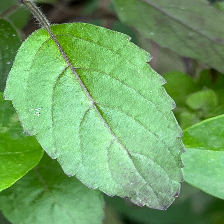
\includegraphics[width=2cm]{images/Introduction/BDML/Inception_V3/IMG_9012_original.png} \\[-1mm]
\scriptsize Ocimum tenuiflorum (BDML) % Original image
\end{tabular}
&
\begin{tabular}[c]{c}
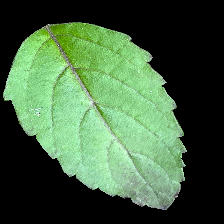
\includegraphics[width=2cm]{images/Introduction/BDML/Inception_V3/IMG_9012_segmented.png} \\[-1mm]
\scriptsize %Segmented image
\end{tabular}
&
\begin{tabular}[c]{c}
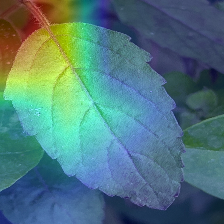
\includegraphics[width=2cm]{images/Introduction/BDML/Inception_V3/IMG_9012_clean.png} \\[-1mm]
\scriptsize LMOS: 0.383 
\end{tabular}
&
\begin{tabular}[c]{c}
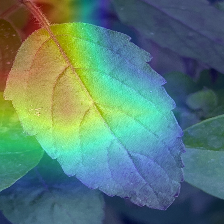
\includegraphics[width=2cm]{images/Introduction/BDML/Inception_V3/IMG_9012_hue.png} \\[-1mm]
\scriptsize LMOS: 0.659 
\end{tabular}
&
\begin{tabular}[c]{c}
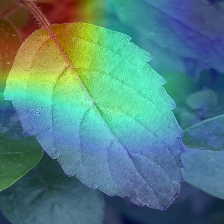
\includegraphics[width=2cm]{images/Introduction/BDML/Inception_V3/IMG_9012_blur.png} \\[-1mm]
\scriptsize LMOS: 0.477
\end{tabular}
&
\begin{tabular}[c]{c}
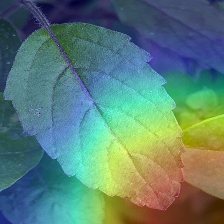
\includegraphics[width=2cm]{images/Introduction/BDML/Inception_V3/IMG_9012_contrast.png} \\[-1mm]
\scriptsize LMOS: 0.390 (wrong prediction)
\end{tabular}
&
\begin{tabular}[c]{c}
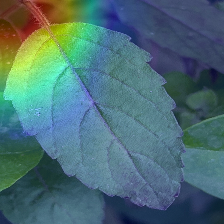
\includegraphics[width=2cm]{images/Introduction/BDML/Inception_V3/IMG_9012_compression.png} \\[-1mm]
\scriptsize LMOS: 0.176
\end{tabular}
\\
\hline

\end{tabular}%
}
\end{table*}








% FLRS  idx = 10
\begin{table*}[htbp]
\centering
\renewcommand{\arraystretch}{1.5}
\caption{Grad-CAM visualization on Flower datasets}
\label{tab:model_robustness}

\resizebox{\textwidth}{!}{%
\begin{tabular}{C{3.5cm} C{2.2cm} C{2.2cm} C{2.2cm} C{2.2cm} C{2.2cm} C{2.2cm} C{2.2cm}}
\hline

\textbf{Model} &
\textbf{Original} &
\textbf{Segmented} &
\textbf{Clean} &
\textbf{Hue} &
\textbf{Blur} &
\textbf{Contrast} &
\textbf{Compression}
\\
\hline

\begin{tabular}[c]{l}
Model: Xception \\
Accuracy: 88.28\% \\
Mean LMOS: 0.6869 \\
ETI: 0.7849 \\
ERI: 0.9308
\end{tabular}
&
\begin{tabular}[c]{c}
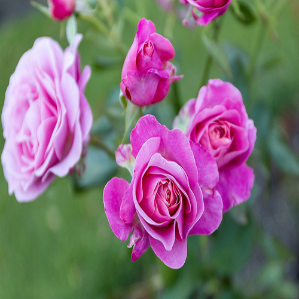
\includegraphics[width=2cm]{images/Introduction/tensorflow_dataset/Xception/11944957684_2cc806276e_original.png} \\[-1mm]
\scriptsize Rose (FLRS) % Original image
\end{tabular}
&
\begin{tabular}[c]{c}

\includegraphics[width=2cm]{images/Introduction/tensorflow_dataset/Xception/11944957684_2cc806276e_segmented.png} \\[-1mm]
\scriptsize %Segmented image
\end{tabular}
&
\begin{tabular}[c]{c}
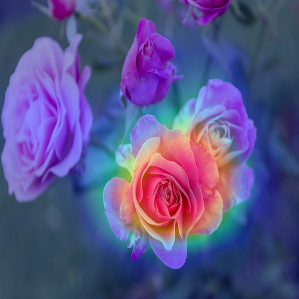
\includegraphics[width=2cm]{images/Introduction/tensorflow_dataset/Xception/11944957684_2cc806276e_clean.png} \\[-1mm]
\scriptsize LMOS: 1.00
\end{tabular}
&
\begin{tabular}[c]{c}
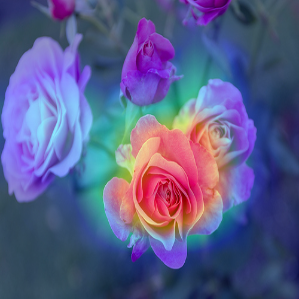
\includegraphics[width=2cm]{images/Introduction/tensorflow_dataset/Xception/11944957684_2cc806276e_hue.png} \\[-1mm]
\scriptsize LMOS: 1.00
\end{tabular}
&
\begin{tabular}[c]{c}
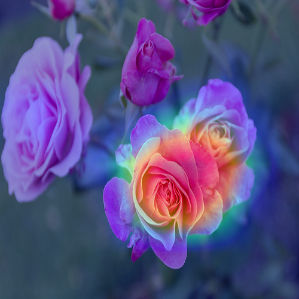
\includegraphics[width=2cm]{images/Introduction/tensorflow_dataset/Xception/11944957684_2cc806276e_blur.png} \\[-1mm]
\scriptsize LMOS: 1.0
\end{tabular}
&
\begin{tabular}[c]{c}
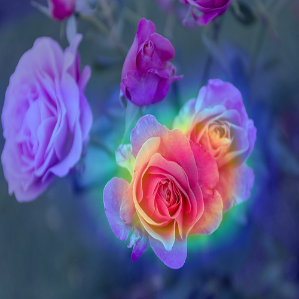
\includegraphics[width=2cm]{images/Introduction/tensorflow_dataset/Xception/11944957684_2cc806276e_contrast.png} \\[-1mm]
\scriptsize LMOS: 1.00
\end{tabular}
&
\begin{tabular}[c]{c}
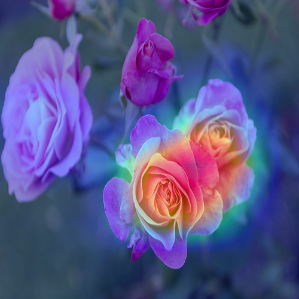
\includegraphics[width=2cm]{images/Introduction/tensorflow_dataset/Xception/11944957684_2cc806276e_compression.png} \\[-1mm]
\scriptsize LMOS: 1.00
\end{tabular}
\\
\hline

\begin{tabular}[c]{l}
Model: Inception V3 \\
Accuracy: 82.29\% \\
Mean LMOS: 0.3749\\
ETI: 0.5989 \\
ERI: 0.8593
\end{tabular}
&
\begin{tabular}[c]{c}
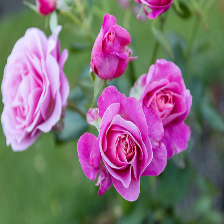
\includegraphics[width=2cm]{images/Introduction/tensorflow_dataset/Inception_V3/11944957684_2cc806276e_original.png} \\[-1mm]
\scriptsize Rose (FLRS) % Original image
\end{tabular}
&
\begin{tabular}[c]{c}

\includegraphics[width=2cm]{images/Introduction/tensorflow_dataset/Inception_V3/11944957684_2cc806276e_segmented.png} \\[-1mm]
\scriptsize %Segmented image
\end{tabular}
&
\begin{tabular}[c]{c}
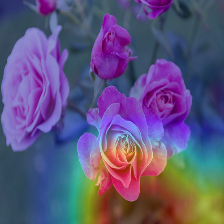
\includegraphics[width=2cm]{images/Introduction/tensorflow_dataset/Inception_V3/11944957684_2cc806276e_clean.png} \\[-1mm]
\scriptsize LMOS: 0.305
\end{tabular}
&
\begin{tabular}[c]{c}
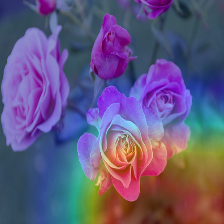
\includegraphics[width=2cm]{images/Introduction/tensorflow_dataset/Inception_V3/11944957684_2cc806276e_hue.png} \\[-1mm]
\scriptsize LMOS: 0.219
\end{tabular}
&
\begin{tabular}[c]{c}
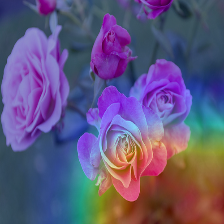
\includegraphics[width=2cm]{images/Introduction/tensorflow_dataset/Inception_V3/11944957684_2cc806276e_blur.png} \\[-1mm]
\scriptsize LMOS: 0.181 
\end{tabular}
&
\begin{tabular}[c]{c}
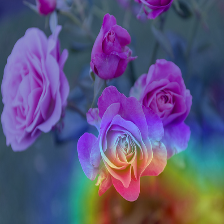
\includegraphics[width=2cm]{images/Introduction/tensorflow_dataset/Inception_V3/11944957684_2cc806276e_contrast.png} \\[-1mm]
\scriptsize LMOS: 0.219 
\end{tabular}
&
\begin{tabular}[c]{c}
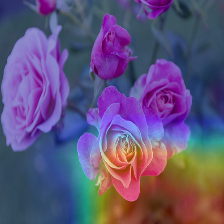
\includegraphics[width=2cm]{images/Introduction/tensorflow_dataset/Inception_V3/11944957684_2cc806276e_compression.png} \\[-1mm]
\scriptsize LMOS: 0.214
\end{tabular}
\\
\hline


\begin{tabular}[c]{l}
Model: Xception \\
Accuracy: 90.32\% \\
Mean LMOS: 0.6029 \\
ETI: 0.7531 \\
ERI: 0.9689
\end{tabular}
&
\begin{tabular}[c]{c}
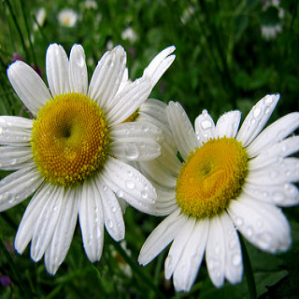
\includegraphics[width=2cm]{images/Introduction/FR/Xception/4668543441_79040ca329_n_original.png} \\[-1mm]
\scriptsize Daisy (FR) % Original image
\end{tabular}
&
\begin{tabular}[c]{c}
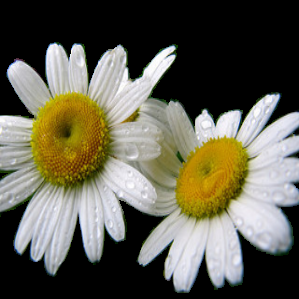
\includegraphics[width=2cm]{images/Introduction/FR/Xception/4668543441_79040ca329_n_segmented.png} \\[-1mm]
\scriptsize %Segmented image
\end{tabular}
&
\begin{tabular}[c]{c}
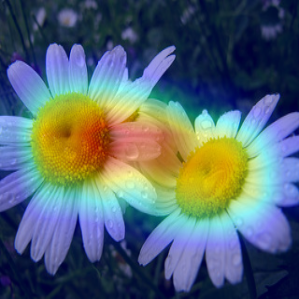
\includegraphics[width=2cm]{images/Introduction/FR/Xception/4668543441_79040ca329_n_clean.png} \\[-1mm]
\scriptsize LMOS: 1.00
\end{tabular}
&
\begin{tabular}[c]{c}
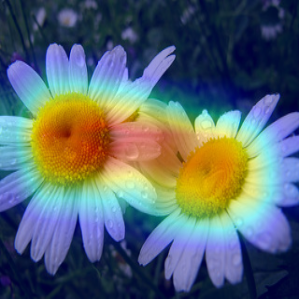
\includegraphics[width=2cm]{images/Introduction/FR/Xception/4668543441_79040ca329_n_hue.png} \\[-1mm]
\scriptsize LMOS: 1.00
\end{tabular}
&
\begin{tabular}[c]{c}
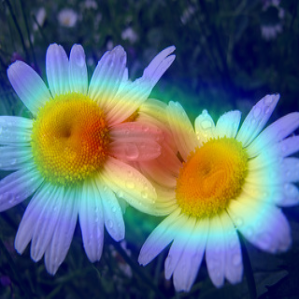
\includegraphics[width=2cm]{images/Introduction/FR/Xception/4668543441_79040ca329_n_blur.png} \\[-1mm]
\scriptsize LMOS: 1.0
\end{tabular}
&
\begin{tabular}[c]{c}
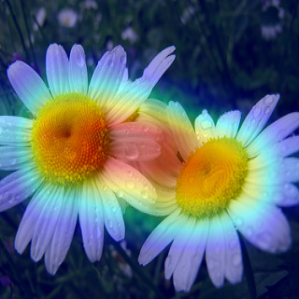
\includegraphics[width=2cm]{images/Introduction/FR/Xception/4668543441_79040ca329_n_contrast.png} \\[-1mm]
\scriptsize LMOS: 1.00
\end{tabular}
&
\begin{tabular}[c]{c}
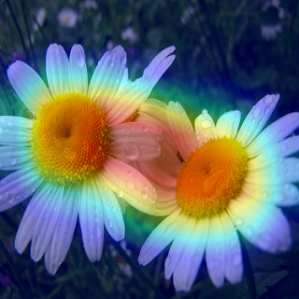
\includegraphics[width=2cm]{images/Introduction/FR/Xception/4668543441_79040ca329_n_compression.png} \\[-1mm]
\scriptsize LMOS: 1.00
\end{tabular}
\\
\hline


\begin{tabular}[c]{l}
Model: Inception V3 \\
Accuracy: 88.25\% \\
Mean LMOS: 0.3063\\
ETI: 0.5944 \\
ERI: 0.8827
\end{tabular}
&
\begin{tabular}[c]{c}
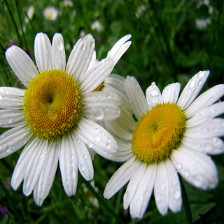
\includegraphics[width=2cm]{images/Introduction/FR/Inception_V3/4668543441_79040ca329_n_original.png} \\[-1mm]
\scriptsize Daisy (FR) % Original image
\end{tabular}
&
\begin{tabular}[c]{c}
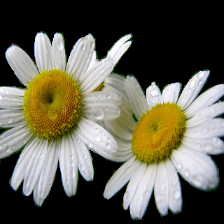
\includegraphics[width=2cm]{images/Introduction/FR/Inception_V3/4668543441_79040ca329_n_segmented.png} \\[-1mm]
\scriptsize %Segmented image
\end{tabular}
&
\begin{tabular}[c]{c}
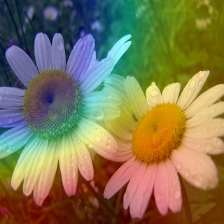
\includegraphics[width=2cm]{images/Introduction/FR/Inception_V3/4668543441_79040ca329_n_clean.png} \\[-1mm]
\scriptsize LMOS: 0.633
\end{tabular}
&
\begin{tabular}[c]{c}
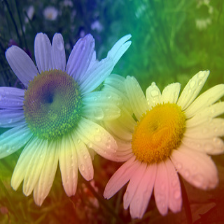
\includegraphics[width=2cm]{images/Introduction/FR/Inception_V3/4668543441_79040ca329_n_hue.png} \\[-1mm]
\scriptsize LMOS: 0.583
\end{tabular}
&
\begin{tabular}[c]{c}
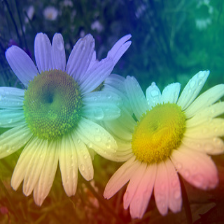
\includegraphics[width=2cm]{images/Introduction/FR/Inception_V3/4668543441_79040ca329_n_blur.png} \\[-1mm]
\scriptsize LMOS: 0.550 
\end{tabular}
&
\begin{tabular}[c]{c}
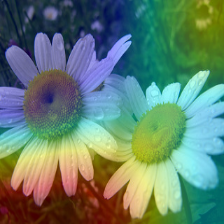
\includegraphics[width=2cm]{images/Introduction/FR/Inception_V3/4668543441_79040ca329_n_contrast.png} \\[-1mm]
\scriptsize LMOS: 0.388 
\end{tabular}
&
\begin{tabular}[c]{c}
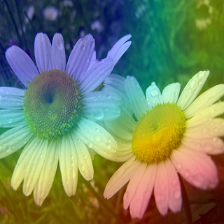
\includegraphics[width=2cm]{images/Introduction/FR/Inception_V3/4668543441_79040ca329_n_compression.png} \\[-1mm]
\scriptsize LMOS: 0.505
\end{tabular}
\\
\hline

\end{tabular}%
}
\end{table*}





    
	---

	\textbf{Two questions that the proposed measures can answer - How trustworty a model is? Trustworty means - predictions are based on real objects in the images. How robust a model is? Robustness means - performance of the model will not degrade under purturbations. }
	
	\zahid{
	To show in exp:
	\begin{itemize}
		\item Acc high but not relaiable - may be low robustness or predictions based on BG. 
		\item a model having high acc but low LMOS and has one or more of the mentioned problems
		\item A model is trustworthy if it has high accuracy and high LMOS - show this. Idea: models with high ACC an high LMOS making more predictions based on objects in images rather than BGs
		\item Show LMOS still works with purturbations and ACC and other traditional measure fails. 
		\item Justify distinctions between EI and RI
		\item Show - traditional measures fail under purturbations but proposed measures hold. 
	\end{itemize}
	}

    
	
	\section{Problem Definition}
	\label{sec:problem_def}
	Let  $\mathcal{D}=\{(x_i,y_i,M_i)\}_{i=1}^{N}$ be a dataset containing $N$ test images, where $x_i\in \mathbb R^{n\times m}$ is the $i$-th image, $y_i$ is its ground-truth label, and $M_i$ is the corresponding ground-truth mask of the target object. 
	%Let $\mathcal{F}$ denote a set of $K$ CNN architectures evaluated on the same test dataset. Here, $\mathcal{F} = \{f_1, f_2, \ldots, f_K\}$. 
	Conventional evaluation methods primarily measure the classification accuracy of a model. 
	Let $acc\in[0,1]$ denote the classification accuracy of a model. 
	
	%Although acc measures predictive performance, it does not indicate whether the model's decision-relevant activation is spatially aligned with the target object. 
	Two CNNs may achieve identical accuracy while relying on substantially different image regions. 
	In particular, a model may achieve high accuracy while its Grad-CAM activation map reveals that the activated regions concentrated outside the target object. 
	Hence, accuracy is insufficient to distinguish models according to their object-focused explanatory behavior.
	
	%We want to quantify the aspect concerning a model's ratianale behind the predictions. 
	%Let $H_{i}$ denotes the Grad-CAM heatmap corresponding to image $x_i$ and prediction $\hat y_i$. 
	%We want to develop a scoring function $\mathrm{LMOS}_i \in[0,1]$ that will measure the ratio between the overlap between the decision-relevant regions of $H_i$ and the ground-truth object mask $M_i$. 
	We seek to quantify the alignment between a model's rationale and its predictions. 
	Let $H_i$ denote the Grad-CAM heatmap corresponding to image $x_i$ and prediction $\hat{y}_i$. 
	We define a scoring function $\mathrm{LMOS}_i \in [0, 1]$ to measure the overlap ratio between the decision-relevant regions of $H_i$ and the ground-truth object mask $M_i$ %and $ L$ is the mean LMOS value across all images.
	%and the total highlighted regions, \(H_{i}\). 
	To indicate model trustworthiness and robustness, we address the following two sub problems in this paper.
	
	Firstly, we want to evaluate CNN models considering both their accuracy ($acc$) and mean object-focused explanation quality ($\mathrm{LMOS}$). 
	Formally, the objective is to develop an evaluation measure $T$ as a function of $acc$ and $\mathrm{LMOS}$: $T = \Psi(acc, \mathrm{LMOS})$. 
	We address this problem by the proposed Explainable Trustworthy Index (ETI).
	
	Secondly, we want to incorporate CNNs behavioural changes in response to perturbations in model evaluation metric. 
	Let $\mathcal{P}=\{p_1,p_2,\ldots,p_P\}$ denote a set of input perturbations. 
	A robust CNN should not only preserve its predictive performance under any changes in $\mathcal{P}$ but also maintain a similar object-focused activation pattern simailar to the model's behavior on the corresponding clean image. 
	%Therefore, accuracy stability and explanation stability need to be considered jointly.
	%Let $acc_{\mathrm{clean}}$ and $acc_{\mathrm{perturbed}}$ denote the classification accuracy of a model on the clean and perturbed test sets, respectively. 
	%Similarly, also let $\mathrm{LMOS}_{\mathrm{clean}}$ and $\mathrm{LMOS}_{\mathrm{perturbed}}$ denote the LMOS values for the clean and perturbed versions of the test set. 
	%The perturbation-specific accuracy stability and LMOS stability are therefore defined as measures of how closely the model preserves its predictive performance and object-focused behavior relative to the clean condition. 
	Let $S_{\mathrm{acc}}$ and $S _ {\mathrm{LMOS}}$ represent the overall accuracy stability (the model's stability to perform under purturbation) and LMOS stability (the model's stability to remain the object-focused for making predictions) of a model. 
	Our second problem is to obtain an evaluation measure $R$ that jointly captures these two forms of stability across the evaluated perturbations: $R = \Phi(S_{\mathrm{acc}},  S_{\mathrm{LMOS}})$. 
	We propose Explainable Robustness Index (ERI) to address this problem. Table \ref{tab:notation} has described each notation clearly.
	
	%Therefore, the overall evaluation problem addressed in this study is to distinguish CNN architectures not only according to how accurately they classify clean images, but also according to whether their decision-relevant activation is aligned with the intended target object and whether both predictive performance and object-focused behavior remain stable under input perturbations. ETI addresses the first aspect on clean inputs, whereas ERI addresses the stability of these properties under perturbations. The two indices are complementary and are not intended to represent the overall trustworthiness or robustness of a CNN across all possible dimensions.

    \begin{table}[t]
	\centering
	\caption{Notation used in the problem formulation.}
	\label{tab:notation}
	\begin{tabular}{ll}
		\toprule
		\textbf{Notation} & \textbf{Description} \\
		\midrule
		$\mathcal{D}$ & Dataset of $N$ images with labels and target masks \\
		$N$ & Number of images in the dataset \\
		$x_i$ & $i$-th input image \\
		$y_i$ & Ground-truth class label of $x_i$ \\
		$\hat{y}_i$ & Predicted class label for $x_i$ \\
		$M_i$ & Ground-truth binary mask of the target object in $x_i$ \\
		$H_i$ & Grad-CAM heatmap for $x_i$ and $\hat{y}_i$ \\
		$\mathrm{LMOS}_i$ & Object-focused localization score for $x_i$ \\
		$\mathrm{LMOS}$ & Mean LMOS over the evaluated dataset \\
		$acc$ & Classification accuracy of a CNN \\
		$\mathcal{P}$ & Set of $P$ input perturbations \\
		$P$ & Number of evaluated perturbations \\
		$S_{\mathrm{acc}}$ & Overall accuracy stability under perturbations \\
		$S_{\mathrm{LMOS}}$ & Overall LMOS stability under perturbations \\
		$T$ & Generic evaluation measure based on $acc$ and $\mathrm{LMOS}$ \\
		$R$ & Generic robustness measure based on $S_{\mathrm{acc}}$ and $S_{\mathrm{LMOS}}$ \\
		$\Psi(\cdot)$ & Function combining accuracy and LMOS \\
		$\Phi(\cdot)$ & Function combining accuracy and LMOS stability \\
		\bottomrule
	\end{tabular}
\end{table}
	
	
	\zahid{add a table of notations here}
	
	\section{System Architecture}
	
	
	\section{Experimental Setup}	
	\subsection{Dataset}
	We have used four publicly available datasets in our empirical study of the proposed evaluation measures: 
	%EgyPLI \cite{r10}, Bdmedileaves \cite{r11}, Flowers \cite{r12} and Flowers Recognition
	%KAGGLE dataset \cite{r13}. 
	
	\begin{itemize}
		\item \textbf{EPLI}: EPLI (introduced as EgyPLI in \cite{r16}) contains 3,588 JPG images of size $256\times256$ pixels.  
		There are images of 8 species including apple, berry, fig, guava, orange, plum, persimmon, and tomato. 
		%, including both normal and diseased leaves. \zahid{are these are images of leaves or the fruits?} 
		%The images were captured under natural uncontrolled environment. 
		%The images are in JPG format and the size is $256\times256$. 
		The dataset is annotated for image‑level classification  \cite{r16}.
		
		\item \textbf{BDML:} BDML(also known as BDMediLeaves \cite{r17}) is a dataset of 2,029 original leaf images (augmented to 38,606) from 10 medicinal plant species. 
		They are captured with an iPhone 13 under natural light at $3024\times 4032$ resolution. 
		This dataset is designed for machine learning‑based species identification. We used the original dataset (not the augmented one) in our experiments \cite{r17}.
		
		\item \textbf{FLRS}: FLRS (or Flowers \cite{r18}) is a large image dataset for flower classification containing 3,670 training images of five flower species including daisies, tulips, sunflowers, dandelions, and roses. 
		It is available through the TensorFlow Datasets (TFDS) collection \cite{r18}. 
		\zahid{what is the resolution of the images in this dataset?}
		
		\item \textbf{FR}:  This kaggle \cite{r19} dataset is very similar to the FLRS dataset above  consisting the same five species (daisies, dandelions, roses, sunflowers, and tulips). 
		However, the kaggle version contains 4,242 JPG images of resulation of $320\times240$ pixels. Although the image classes are the same as FLRS, the image samples are different.  This repository was also used in previous research \cite {r20, r21}.
		\zahid{is this different than the above FLRS?}
	\end{itemize}
	
	\zahid{Specific difference between FLRS and KFLR}.
	
	\noindent
	\textbf{Dataset preparation.} 
	The BDML dataset is already splitted into training, validation and testing sets. We split the other three datasets into training, validation and test subsets with an approximate ratio of $80\%$, $10\%$ and $10\%$. 
	Table \ref{tab:classwise_dataset_distribution} presents the class-wise training, validation, and test splits. 
	\zahid{did you preserve the class distributions in the three splits?}
		
	\zahid{did you do this? or already in the sources?}
	To simplify explainability and localization analysis, the test images have been manually annotated to generate corresponding JSON files. 
	These JSON annotations describe the polygonal boundaries of the target leaf in each image. 
	The JSON files have been converted into binary masks. 
	Here, each mask represents only the target leaf region and excludes the background and other objects in the scene.
	
	\begin{table}[t]
	\centering
	\caption{Class-wise distribution of the experimental datasets.}
	\label{tab:classwise_dataset_distribution}
	\small % Slightly reduces font size to fit neatly within column margins if needed
	\begin{tabular}{l cccc}
			\toprule
			\textbf{Dataset / Class} & \textbf{Total} & \textbf{Train} & \textbf{Val} & \textbf{Test} \\
			\midrule
			\multicolumn{5}{l}{\textit{EgyPLI}} \\
			Apple     & 519  & 415  & 52  & 52  \\
			Berry     & 340  & 272  & 34  & 34  \\
			Fig           & 508  & 406  & 50  & 52  \\
			Guava     & 520  & 416  & 52  & 52  \\
			Orange    & 547  & 437  & 55  & 55  \\
			Plum      & 468  & 374  & 47  & 47  \\
			Persimmon & 527  & 421  & 53  & 53  \\
			Tomato    & 159  & 127  & 16  & 16  \\
			\cmidrule(lr){2-5}
			\textbf{Subtotal} & \textbf{3,588} & \textbf{2,868} & \textbf{359} & \textbf{361} \\
			
			\midrule
			\multicolumn{5}{l}{\textit{Flowers (TFDS)}} \\
			Daisy      & 633  & 506  & 64  & 63  \\
			Dandelion  & 898  & 718  & 90  & 90  \\
			Roses      & 641  & 512  & 64  & 65  \\
			Sunflowers & 699  & 560  & 70  & 69  \\
			Tulips     & 799  & 639  & 80  & 80  \\
			\cmidrule(lr){2-5}
			\textbf{Subtotal} & \textbf{3,670} & \textbf{2,935} & \textbf{368} & \textbf{367} \\
			
			\midrule
			\multicolumn{5}{l}{\textit{Flowers Recognition}} \\
			Daisy      & 764  & 611  & 76  & 77  \\
			Dandelion  & 1052 & 842  & 105 & 105 \\
			Roses      & 784  & 627  & 78  & 79  \\
			Sunflowers & 733  & 586  & 73  & 74  \\
			Tulips     & 984  & 787  & 98  & 99  \\
			\cmidrule(lr){2-5}
			\textbf{Subtotal} & \textbf{4,317} & \textbf{3,453} & \textbf{430} & \textbf{434} \\
			
			\bottomrule
		\end{tabular}
\end{table}
	

	%\subsection{Dataset Distribution}	
		
	\subsection{Baseline models and evaluation metrics.}
	TBD
	
	\subsection{Classification Performance}
	%\subsection{Creating JSON files of test images }
	% moved above in dataset prep. section
	
	\subsection{Implementation of the Proposed Metrics}
	Both of the proposed TI and RI metrics use LMOS score. 
	LMOS measure the consistency between model-generated explanations and ground-truth object regions. 
	\zahid{One liner on TI and RI to be added here}
	We briefly describe the implementation details of these metrics below. 
	
	 %\noindent
	\subsubsection{Localization Mask Overlap Score (LMOS).} 
	\zahid{need to say LMOS is an instance specific (or loca) measure. Other metrics e.g., acc - is a global measure - indicate overall perf. Thats why we use $\overline{LMOS}$ in TI definition, just need to say it outloud here}
	LMOS calculates how much a model focuses on true object regions (instead of backgrouds) for prediction. 
	Let $H \in \mathbb{R}^{h \times w}$ denote the Grad-CAM heatmap generated from the last convolutional layer of a network. 
	$H$ is resized to the model's input image size.  \zahid{if H is size how can it be $ \mathbb{R}^{h \times w}$??}
	The resized heatmap size is $299 \times 299$ for Xception, $224\times224$ for other models. 
	A binary attention map is obtained from $H$ by thresholding:
	%\begin{equation}
	$$\hat H (i,j) = \mathbb{I}\left( \mathrm{Resize}(H)(i,j) > \tau \right)$$
	%\end{equation}
	where $\mathbb{I}(\cdot)$ is an indicator function and $\tau$ is the threshold \zahid{to or for??}. 
	%We set $\tau=0.7$ as we consider only red and yellow pixels to calculate LMOS as those pixels are the most activated and decision-relevant for predictions. 
	We set $\tau=0.7$ \zahid{why? through experiments or what? how $\tau=0.7$ restricts to yellow and red pixels??} to restrict our LMOS calculations to red and yellow pixels, as the red and yelow pixels exhibit the highest activation levels in model predictions. 
	Hence, $\hat{H}(i,j)$ is a binary mask representing the activated decision-relevant regions. 
	
	%Masks have been created from JSON files of test images and resized into the input image size (299*299 for Xception, 224*224 for others). 
	% use h and w to express height and width every where
	%
	%Here, object pixel values are assigned 1, others 0. already said since it is binary
	
	LMOS is defined as the ratio of activated decision-relevant regions inside the object region and the total activated decision-relevant regions. 
	Mathematically:
	\begin{equation}
		\label{eq:lmos}
		\mathrm{LMOS}  \frac{\sum_{i=1}^{h}\sum_{j=1}^{w} \hat{h}(i,j)\, M(i,j)} {\sum_{i=1}^{h}\sum_{j=1}^{w} \hat{H}(i,j)}
	\end{equation}
	where $M \in \{0,1\}^{h \times w}$ denote the resized ground-truth binary segmentation mask.  
	%We have derived the mean LMOS, L for all test images. 
	\zahid{waht is L here? what is $\hat h$ here?}
	
	\zahid{how do we get M???}
	
	\subsubsection{Trustworthy Index (TI)}
	\label{sec:implementaiton_TI}
	In this article, we propose Trustworthy Index (TI) to measure trustworthiness of a CNN model's predictions. 
	We combine the accuracy, explainable consistency and the mean LMOS (Eq. \ref{eq:lmos}) to define TI. 
	
	Let $acc$ denote the classification accuracy of a model on test set and $\overline{\mathrm{LMOS}}$ denote the mean LMOS scores across the same test samples. 
	We define TI defined as follows:
	%\[
	$$\mathrm{TI} = \frac{acc + \overline{\mathrm{LMOS}}}{2}.$$
	%\]
	
	In this study, both $acc$ and $\mathrm{LMOS}$ are equally important and are normalized to the range $[0,1]$.
	% and represent complementary components of model reliability. 
	$acc$ measures predictive performance, whereas $\mathrm{LMOS}$ measures the mean explanation consistency with the target object. 
	%Since neither component alone is sufficient to estimate trustworthiness, 
	We provide equal weighting to both components to avoid favoring either predictive performance or explanatory quality. \zahid{need to rewrite}
	
	%\subsubsection{Ablation Study}
	\noindent
	\textbf{Variations of TI}. 
	To demonstrate the impact of LMOS and $acc$ on the proposed TI, we have calculated two variants of TI as folllows:
	$$\mathrm{TI}_{\text{w/o LMOS}} = \frac{\text{acc}}{2}, \quad \mathrm{TI}_{\text{w/o acc}} = \frac{\text{LMOS}}{2}.$$
	
	\subsubsection{Robustness Index (RI)}
	We estimate the robustness of a model by measure its' performance deviation under purturbation in the test datasets.  
	%To evaluate performance robustness against input perturbations, we compute Accuracy Stability ($S_{\rm{acc}}$)  \zahid{if not introduced by you cite}, which measures the consistency between the classification accuracy on perturbed images and the baseline accuracy on clean test images.
	Let $acc_c$ denote the accuracy of a model on a clean test dataset (not purturbed) and $acc_p$ denote the accuracy obtained on the test set after applying a specific perturbation $p$ (see Sec. \ref{sec:perturbation_methods} for all the purturbation methods used in this research). 
	We intorduce the Accuracy Stability ($S_{\rm{acc}}$) score \zahid{if not introduced by you cite} under a specific perturbation $p$ as:
	%begin{equation}
	$$	S_{\mathrm{acc}}^{p} = 1 - \frac{ | acc_c - acc_p | }
	{acc_c + acc_p + \epsilon}$$
	%\end{equation}
	where $\epsilon$ is a small positive constant introduced to avoid division by zero error. 
	A higher value of $S_{\mathrm{acc}}^p$ indicates that the model's performance is more consistent under the corresponding perturbed condition $p$. 
	
	To estimate an overall measure of $S_{\mathrm{acc}}$, we compute $S_{\mathrm{acc}}^p$ across all $p \in P$ where $P$ is the set of all purturbation methods used in the experiments, see Section \ref{sec:perturbation_methods} and take the mean of all $S_{\mathrm{acc}}^p$. 
	This can be defined as:
	%\begin{equation}
	$$\overline{S}_{\text{acc}} = \frac{1}{|P|} \sum_{p=1}^{|P|} S_{\text{acc}}^{p}$$
	%\end{equation}
	%where $S_{\text{acc}}^{(p)}$ denotes the accuracy stability under the $p$-th perturbation and $P$ is the total %number of evaluated perturbations. In this study, $P=9$.
	
	%\zahid{proposed measures EI and RI. they use LMOS. What are the additional measures - stability ??? Need to clarify.}
	
	\textbf{Similarly, we introduce LMOS Stability to measures how closely a model's object reliance under perturbation remains to its object reliance on clean images.
	To evaluate the robustness under input perturbations, we have measured the stability of LMOS when input images are perturbed.} \zahid{need rewriting}

	For each test sample, we have computed LMOS for both the original image and its perturbed version.  
	Let $N$ be the number of test samples in a test set. 
	Let $LMOS_{\text{clean}}$ denote the LMOS value computed from an original image and $LMOS_{\text{perturbed}}$ denote the LMOS value computed from the corresponding perturbed image.
	
	To quantify the consistency between these two values, we define the LMOS stability under a perturbation:
	%\begin{equation}
	$$S_{\textrm{LMOS}} = 1 - \frac{|LMOS_{\textrm{clean}} - LMOS_{\textrm{perturbed}}|}{LMOS_{\textrm{clean}} + LMOS_{\textrm{perturbed}} + \epsilon}$$, 
	%\end{equation}
	where $\epsilon$ is a small constant to avoid division by zero error. 
	
	\zahid{why not the denominator is using abs values?}
	
	A higher value of $S_{\text{LMOS}}$ indicates that the model's reliance on the focus object remains more consistent under the corresponding perturbation. The LMOS stability under a perturbation $p$ is calculated as an average across all $N$ test samples as:
	
	\begin{equation}
		{S}_{\text{LMOS}}^{(p)}
		=
		\frac{1}{N}
		\sum_{i=1}^{N}
		S_{\text{LMOS},i}^{(p)}
	\end{equation}
	
	where $S_{\text{LMOS},i}^{(p)}$ denotes the LMOS stability of the $i$-th test sample under the perturbation $p$, and $N$ represents the total number of test samples.
	
	To obtain an overall measure of LMOS stability across all evaluated perturbations, the perturbation-specific LMOS stability scores are subsequently averaged as:
	
	\begin{equation}
		\overline{S}_{\text{LMOS}}
		=
		\frac{1}{P}
		\sum_{p=1}^{P}
		{S}_{\text{LMOS}}^{(p)}.
	\end{equation}
	
	where $P$ denotes the total number of evaluated perturbations. In this study, $P=9$.
	
	
	
	%  ------ Needs checking--------------
	To jointly evaluate the robustness of both classification performance and explainability under input perturbations, we have proposed the \textit{Explainable Robustness Index} (ERI). Unlike accuracy stability and LMOS stability, which separately assess the consistency of predictive performance and model localization behavior, ERI provides a unified measure of robustness by combining the accuracy stability and LMOS stability.
	
	Let ${s}_{\text{acc}}^{{p}}$ be accuracy stability and ${s}_{\text{LMOS}}^{{p}}$ be LMOS stability under perturbation p. Now, ERI under perturbation p is calculated as:
	
	
	\begin{equation}
		ERI^{{p}} =
		\frac{
			{S}_{\text{acc}}^{{p}}
			+
			{S}_{\text{LMOS}}^{{p}}
		}{2}.
	\end{equation}
	
	Let $\overline{S}_{\text{acc}}$ denote the overall accuracy stability and $\overline{S}_{\text{LMOS}}$ denote the overall LMOS stability, both obtained by averaging their corresponding perturbation-specific stability scores across the $P$ evaluated perturbations. The proposed ERI is defined as:
	
	\begin{equation}
		ERI =
		\frac{
			\overline{S}_{\text{acc}}
			+
			\overline{S}_{\text{LMOS}}
		}{2}.
	\end{equation}
	
	Here, $\overline{S}_{\text{acc}}$ represents the overall consistency of classification accuracy between clean and perturbed inputs, while $\overline{S}_{\text{LMOS}}$ represents the overall consistency of the model's reliance on the focus object under perturbations. Therefore, ERI jointly captures two complementary dimensions of robustness: \textit{predictive stability} and \textit{explanatory stability}.
	
	Since both component scores are bounded in the same range, the resulting ERI also provides a normalized measure of overall robustness. A higher ERI indicates that a model simultaneously maintains its classification performance and preserves its object-focused behavior across the evaluated perturbations. Conversely, a lower ERI indicates that the model exhibits greater instability in one or both dimensions.
	
	%\subsubsection{Ablation Study}
	\noindent
	\textbf{Variations of RI.}
	To analyze the contribution of the individual components of RI (i.e., $S_{acc}$ and $S_{\text{LMOS}}$), we calculate two variants by removing one component at a time:
	$$\mathrm{RI}_{\text{w/o LMOS}} = \frac{\overline{S}_{\text{acc}}}{2}, 
	\quad 
	\mathrm{RI}_{\text{w/o acc}} = \frac{\overline{S}_{\text{LMOS}}}{2}.$$

	
	%\mathrm{LMOS}
	
	%% -- not processed yet
	
	
%	\subsubsection{LMOS (Localization Mask Overlap Score) }
%	\subsubsection{Accuracy Stability }
%	\subsubsection{LMOS Stability Under Perturbations }
	
	\subsection{Grad-CAM Visualization}
	Grad-CAM visualization shows that CNN models often	predictcorrectlybuttheysometimesrelyonthebackground
	or non-object regions. Besides, under perturbations, their	relianceon objectpixels hugely changes. 
	\zahid{it is not necessary here. We may include the implemenation of grad-cam in the method implementation section above}
	
	\subsection{Perturbation methods}
	\label{sec:perturbation_methods}
	To evaluate the robustness of the proposed framework under distribution shifts and common image corruptions, we have applied nine image perturbation methods to the test set. 
	%As summarized in Table~\ref{tab:perturbations}, 
	\zahid{if anything in the table is missing below, add it in the corresponding bullet}
	%These perturbations simulate realistic degradations that may occur during image acquisition, compression, transmission, or environmental variation. 
	The perturbation parameters have been fixed across all experiments to ensure reproducibility and enable fair comparisons among different CNN architectures. 
	The details of the perturbations are given below: \zahid{missing references here. Add 1 or more references to papers applying these for the same reason? i.e., evaluation under purturbation}
	
	\begin{itemize}
		\item \textbf{Gaussian Blur:} Applied using a $5 \times 5$ kernel to simulate the loss of fine spatial details caused by defocus or low-quality imaging conditions.
		
		\item \textbf{Gaussian Noise:} Additive Gaussian noise with zero mean and standard deviation 0.05 has been introduced to model sensor noise and random intensity fluctuations.
		
		\item \textbf{Brightness Adjustment:} Increased by adding a constant value of 0.2 to normalized pixel intensities, after which values have been clipped to the valid range $[0,1]$.
		
		% hue shift was 15, made it 10 as in code
		\item \textbf{Hue Shift:} Hue values in the HSV color space have been shifted by 15 units while preserving the saturation and value channels, simulating color variations caused by illumination or camera characteristics.
		
		% times 1 but here was 0.5
		\item \textbf{Contrast Adjustment:} Modified using mean-centered linear scaling: $ I' = (I - \mu_I)\times 0.5 + \mu_I$, where $I$ denotes the input image and $\mu_I$ represents the mean pixel intensity (computed per channel). 
		The resulting values have been clipped to the range $[0,1]$.
		
		% its gamma = 1 in code, here was 2
		\item \textbf{Gamma Correction:} Nonlinear illumination changes have been simulated using gamma correction: $I' = I^{2.0}$, where pixel intensities have been raised to the power of $\gamma = 2.0$.
		
		\item \textbf{Motion Blur:} Simulated using a $7 \times 7$ horizontal averaging kernel to emulate camera or object motion during image acquisition.
		
		\item \textbf{JPEG Compression:} Artifacts have been introduced by encoding and decoding the images with a quality factor of 30, simulating degradation due to lossy storage or transmission.
		
		\item \textbf{Random Occlusion:} A randomly positioned rectangular region corresponding to 20\% of the image height and 20\% of the image width has been masked by setting its pixel values to zero, thereby simulating partial object occlusion.
	\end{itemize}
	
	
	\subsection{Training Configurations}
	We used TensorFlow/Keras on the Kaggle \zahid{cite kaggle} environment with two NVIDIA Tesla T4 GPUs to trainining and evaluation of all the CNN models in our experiments. 
	The training configuration has followed the settings adopted in the original EgyPLI study\cite{r10}. \zahid{what are these? please specify. is it only for EgyPLI or all 4 datasets??}
	The custom CNN was trained from scratch, while other models have been initialized with ImageNet-pretrained weights \zahid{cite here} and their backbone layers have been frozen.
	
	For the pretrained models, the original classification heads have been removed and replaced with a common classification head consisting of Global Average Pooling \zahid{cite}, a dropout layer \zahid{cite} with dropout rate 0.3, a fully connected layer with 128 ReLU units \zahid{cite}, and the final softmax layer has been configured according to the number of classes in each dataset.
	%The custom CNN has followed its original convolutional architecture. 
	The Adam optimiser \zahid{cite} has been used with a learning rate of $5\times10^{-5}$ and categorical cross-entropy loss \zahid{arg1} in all model optimizations.
	%We have used TensorFlow/Keras Functional API, while the original EgyPLI research used the sequential API. This implementation choice does not alter the underlying CNN architectures or their corresponding backbone configurations.
	
	%The trained models have been subsequently evaluated on clean and perturbed test images. Their classification accuracy and Grad-CAM-based LMOS have been used to calculate accuracy stability, LMOS stability, ETI, and ERI.

	\section{Result and Discussion}
	\subsection{Grad-CAM Visualization}
	\label{sec:gradcam_visualization}
	\subsubsection{Threshold Justification}
	\label{sec:threshold_justification}
	
	\subsection{Explainable Trustworthiness Index (ETI)}
	
	\subsection{Explainable Robustness Index (ERI)}
	\noindent\textbf{EgyPLI.} XXXXXX
	%\subsubsection{EgyPLI}
	\subsubsection{BDMediLeaves}
	\subsubsection{Flowers}
	\subsubsection{Flowers Recognition KAGGLE Dataset}
	
	\subsection{Cross-Dataset Analysis}
	
	%\subsection{Ablation Study}
	%\subsubsection{}
	%\subsubsection{}
	
	\section{Related Works}
Javed et al. introduced two approaches: a Bayesian approximation
via Monte Carlo Dropout and the nonparametric Conformal Prediction framework to measure uncertainty \cite{r22}. Although CNN models are excellent for classification, their predictions are often wrong but overconfident. If wrong predictions receive high confidence, the models are overconfident and difficult to trust. These models suffer from poor calibration. Their research indicates that accuracy alone cannot make a model reliable. Recent studies have proposed trustworthiness metrics based on uncertainty estimation and failure detection. Ao et al. \cite{r23} proposed the Excess Area Under the Optimal Risk-Coverage Curve, E-AUoptRC, to evaluate model performance under the risk–coverage (RC) framework. They also introduced the Trust Index (TI), which displays model performance at the optimal coverage point and serves as a complementary metric to overall accuracy. E-AUoptRC and TI provide more trustworthiness of CNN models than other indices/metrics. Nastoska et al. proposed frameworks and metrics to evaluate AI trustworthiness, including fairness, transparency, privacy, and security\cite{r24}. They experimented with various frameworks such as the NIST AI Risk Management Framework (AI RMF), the AI Trust Framework and Maturity Model (AI-TMM), and ISO/IEC standards. Their study includes a comparative analysis of existing standards and their applications in the industry to describe theirabout generalizing effectiveness. Pal et al. proposed the Trust-Aware Explainable Artificial Intelligence (TAXAI) framework. It introduces a quantitative Trust Index for evaluating explainable AI systems in clinical applications\cite{r25}. The framework combines algorithmic transparency, interpretability alignment, and compliance-oriented reliability into a unique trust evaluation model. It is not similar to traditional XAI methods that primarily generate explanations. In contrast, TAXAI focuses on measuring the trustworthiness and reliability of explanations through a normalized trust score.

Zhang et al. proposed AR2, a repair method to improve robustness to corruption without changing the architecture. It aligns the class activation maps (CAMs) for clean and corrupted images and encourages the model to maintain consistency  \cite{r26}. Although AR2 enhances robustness under perturbations, it does not provide any explainable score or index under various perturbations. In contrast, our proposed Explainable Robustness Index (ERI) directly measures the stability of Grad-CAM explanations under perturbations. It provides an explainability-based robustness evaluation. Hendrycks and Dietterich \cite{r27} introduced ImageNet-C and ImageNet-P. Their research evaluates performance under corruption and perturbations. They found negligible changes under corruption from AlexNet to ResNet classifiers. This research calculates performance degradation under distribution shifts but does not assess the stability of model explanations.  Su et al. evaluated the robustness of deep image classification models against various perturbations and demonstrated that high classification accuracy does not necessarily imply high robustness \cite{r28}. This work motivated us to investigate robustness beyond predictive accuracy. Taori et al. defined robustness during natural distribution shifts and emphasized that robustness should be evaluated separately from standard predictive accuracy \cite{r29}. This work further motivated us to evaluate robustness beyond predictive accuracy. Hendrycks et al. proposed AugMix, a data-processing method designed to improve the robustness of image classification models under common corruptions while maintaining performance on clean images \cite{r30}. This research is very motivating for our evaluation of robustness beyond standard predictive accuracy. Schneider et al. evaluated robustness under common image corruptions and showed that covariate-shift adaptation using corrupted test samples can substantially improve model performance under such distribution shifts \cite{r31}. Guo et al. proposed a model robustness evaluation framework \cite{r32}. It contains 23 comprehensive and rigorous metrics. These metrics consider two key aspects of adversarial learning: data and model.

Bassi et al. demonstrated the impact of background on the model's decision \cite {r11}. Background may cause shortcut learning. Layer-wise Relevance Propagation (LRP) explores the model's decision. They revealed that background bias influence on deep learning models can be minimized by LRP heatmaps without increasing computation cost. By injecting synthetic bias in the image's background, they compared their approach to eight state-of-the-art DNNs. Their approach remained more robust.  Grad-CAM and saliency-based methods have been widely utilized to interpret CNN-based classification systems in various sectors, such as plant disease detection. They provide trustworthiness and important insights for decision-making and predictions\cite{r33}. Attention-based and explainability-guided CNN architectures have been widely explored in recent applications. For example, Singh et al. have proposed CBAM-enhanced VGG16 models for plant leaf disease classification. They presented the effectiveness of their research through comprehensive evaluation and interpretability analysis, such as Grad-CAM, Grad-CAM++, and Layer-wise Relevance Propagation (LRP), to make the system more transparent and reliable for smart farming. \cite{r34}. Shawon et al. highlight the growing application of explainable AI techniques such as Grad-CAM, SHAP, and LIME in plant disease detection. They emphasize concerns about generalizing models under real-world conditions and environmental variability, although they provide high accuracy\cite{r35}. However, these works primarily focus on applying interpretability methods rather than quantitatively evaluating explanation quality or robustness, which motivates the need for metrics such as ERI and ETI. A significant problem of Explainable AI is the unavailability of quantifiable metrics to evaluate or measure explanation quality. Rahimiaghdam and Alemdar addressed the issue and proposed evaluative and quantitative metrics of explanation quality in medical imaging \cite{r36}. Baniecki.
et al. expressed the quality of classifiers as the consistency of explanations and ground truth/segmentation masks. They proposed a framework that evaluates robustness by combining deep neural networks with explanations. Similar tasks are widely used in medical imaging. They introduced a fine-tuning approach that aligns model–explanation pipelines with ground truth. \cite{r37}.  Repetto et al. evaluated the robustness of ExAI methods under various perturbations. They systematically measured the stability of ExAI techniques against both natural noise and adversarial manipulations that change explanations but not predictions. Finally, they introduced some evaluative metrics and proposed a protocol to assess the reliability of ExAI methods\cite{r38}. Zheng et al. proposed a spurious bias
mitigation framework, ShortcutProbe\cite{r39}. Here, there is no need for annotation and labeling. ShortcutProbe detects prediction shortcuts that may lessen robustness. The models were retrained again to become invariant to these shortcuts and more robust.  Guidotti et al. propose an approach that allows evaluating the local explanation methods using ground-truth explanations \cite{r40}. We have been motivated by this ground-truth-based evaluation perspective to quantify the spatial alignment between Grad-CAM evidence and ground-truth object regions, leading to the proposed Localization Mask Overlap Score (LMOS). Fong and Vedaldi proposed a general framework that can learn different kinds of explanations for any black-box algorithm and another framework to find the image region most responsible for a classifier decision \cite{r41}. Kim et al. attempted to find out the gap between classification and localization in weakly supervised object localization and showed that CAM-based methods tend to emphasize the most discriminative object parts rather than the complete object region \cite{r42}.



	
	\section{Conclusion}     
	\label{sec:conclusion}
	
	
	
	\section*{Data and Code availability}
	
	Supplementary code and data (including \texttt{.json} files and
	\texttt{.keras} files) associated with this research are available at:
	
	\url{https://github.com/ragib1996/ETI_ERI}
	
	\printcredits
	
	
	\section*{Acknowledgments}
	
	\section*{Disclosure statement}
	
	\section*{Funding}
	
	
	%\bibliographystyle{cas-model2-names}
	\bibliographystyle{ieeetr}
	
	% Loading bibliography database
	\bibliography{cas-refs}
	
\end{document}

